\chapter{The Large Hadron Collider} \label{chap:lhc}

Lying an average of 100 meters under the Swiss / French border, the 26.7
kilometer circumference Large Hadron Collider (LHC) is the world's largest piece
of scientific apparatus built to date \cite{Brüning:782076, Evans:2008zzb}.
This apparatus is used to produce proton and heavy ion collisions for
observation by the four major experiments at the LHC: ATLAS, CMS, LHCb, and
ALICE.  The system was designed for a maximum center-of-mass energy of
$\sqrt{s} = 14$ TeV and a peak instantaneous luminosity of $L = 10^{34} $cm$^{-2} $s$^{-1}$.  

The first LHC workshop was held in 1984 in Lausanne at the European
Organization for Nuclear Research (CERN) \cite{LlewellynSmith:2014lmn}.  The
nearly 30-year-old case for a machine that would push towards the discovery of
the elusive Higgs Boson was presented using the existing CERN accelerator
facilities and the Large Electron Positron (LEP) Collider tunnel. The proposal
became reality on September 10, 2008 when the first proton beams were
circulated, only to have calamity strike 9 days later in the form of a
catastrophic electrical fault \cite{EDMS:973073}. The repairs and improvements
lasted until November 2009 when the LHC restarted.  Since then, this modern
marvel has worked wonderfully and, as hoped, lead to the discovery of the Higgs
Boson by the ATLAS and CMS collaborations, announced on July 4th, 2012
\cite{Aad:2012tfa, Chatrchyan:2012xdj, higgs_announcement}.

The following  chapter provides a brief introduction to the world's most
powerful accelerator starting with the little red bottle of hydrogen, and
ending with the interaction point where protons collide at the highest energies
ever produced by humans.

\section{Particle Injection Chain} \label{sec:lhc:injection}

\begin{figure}[!htbp] 
  \begin{center}
    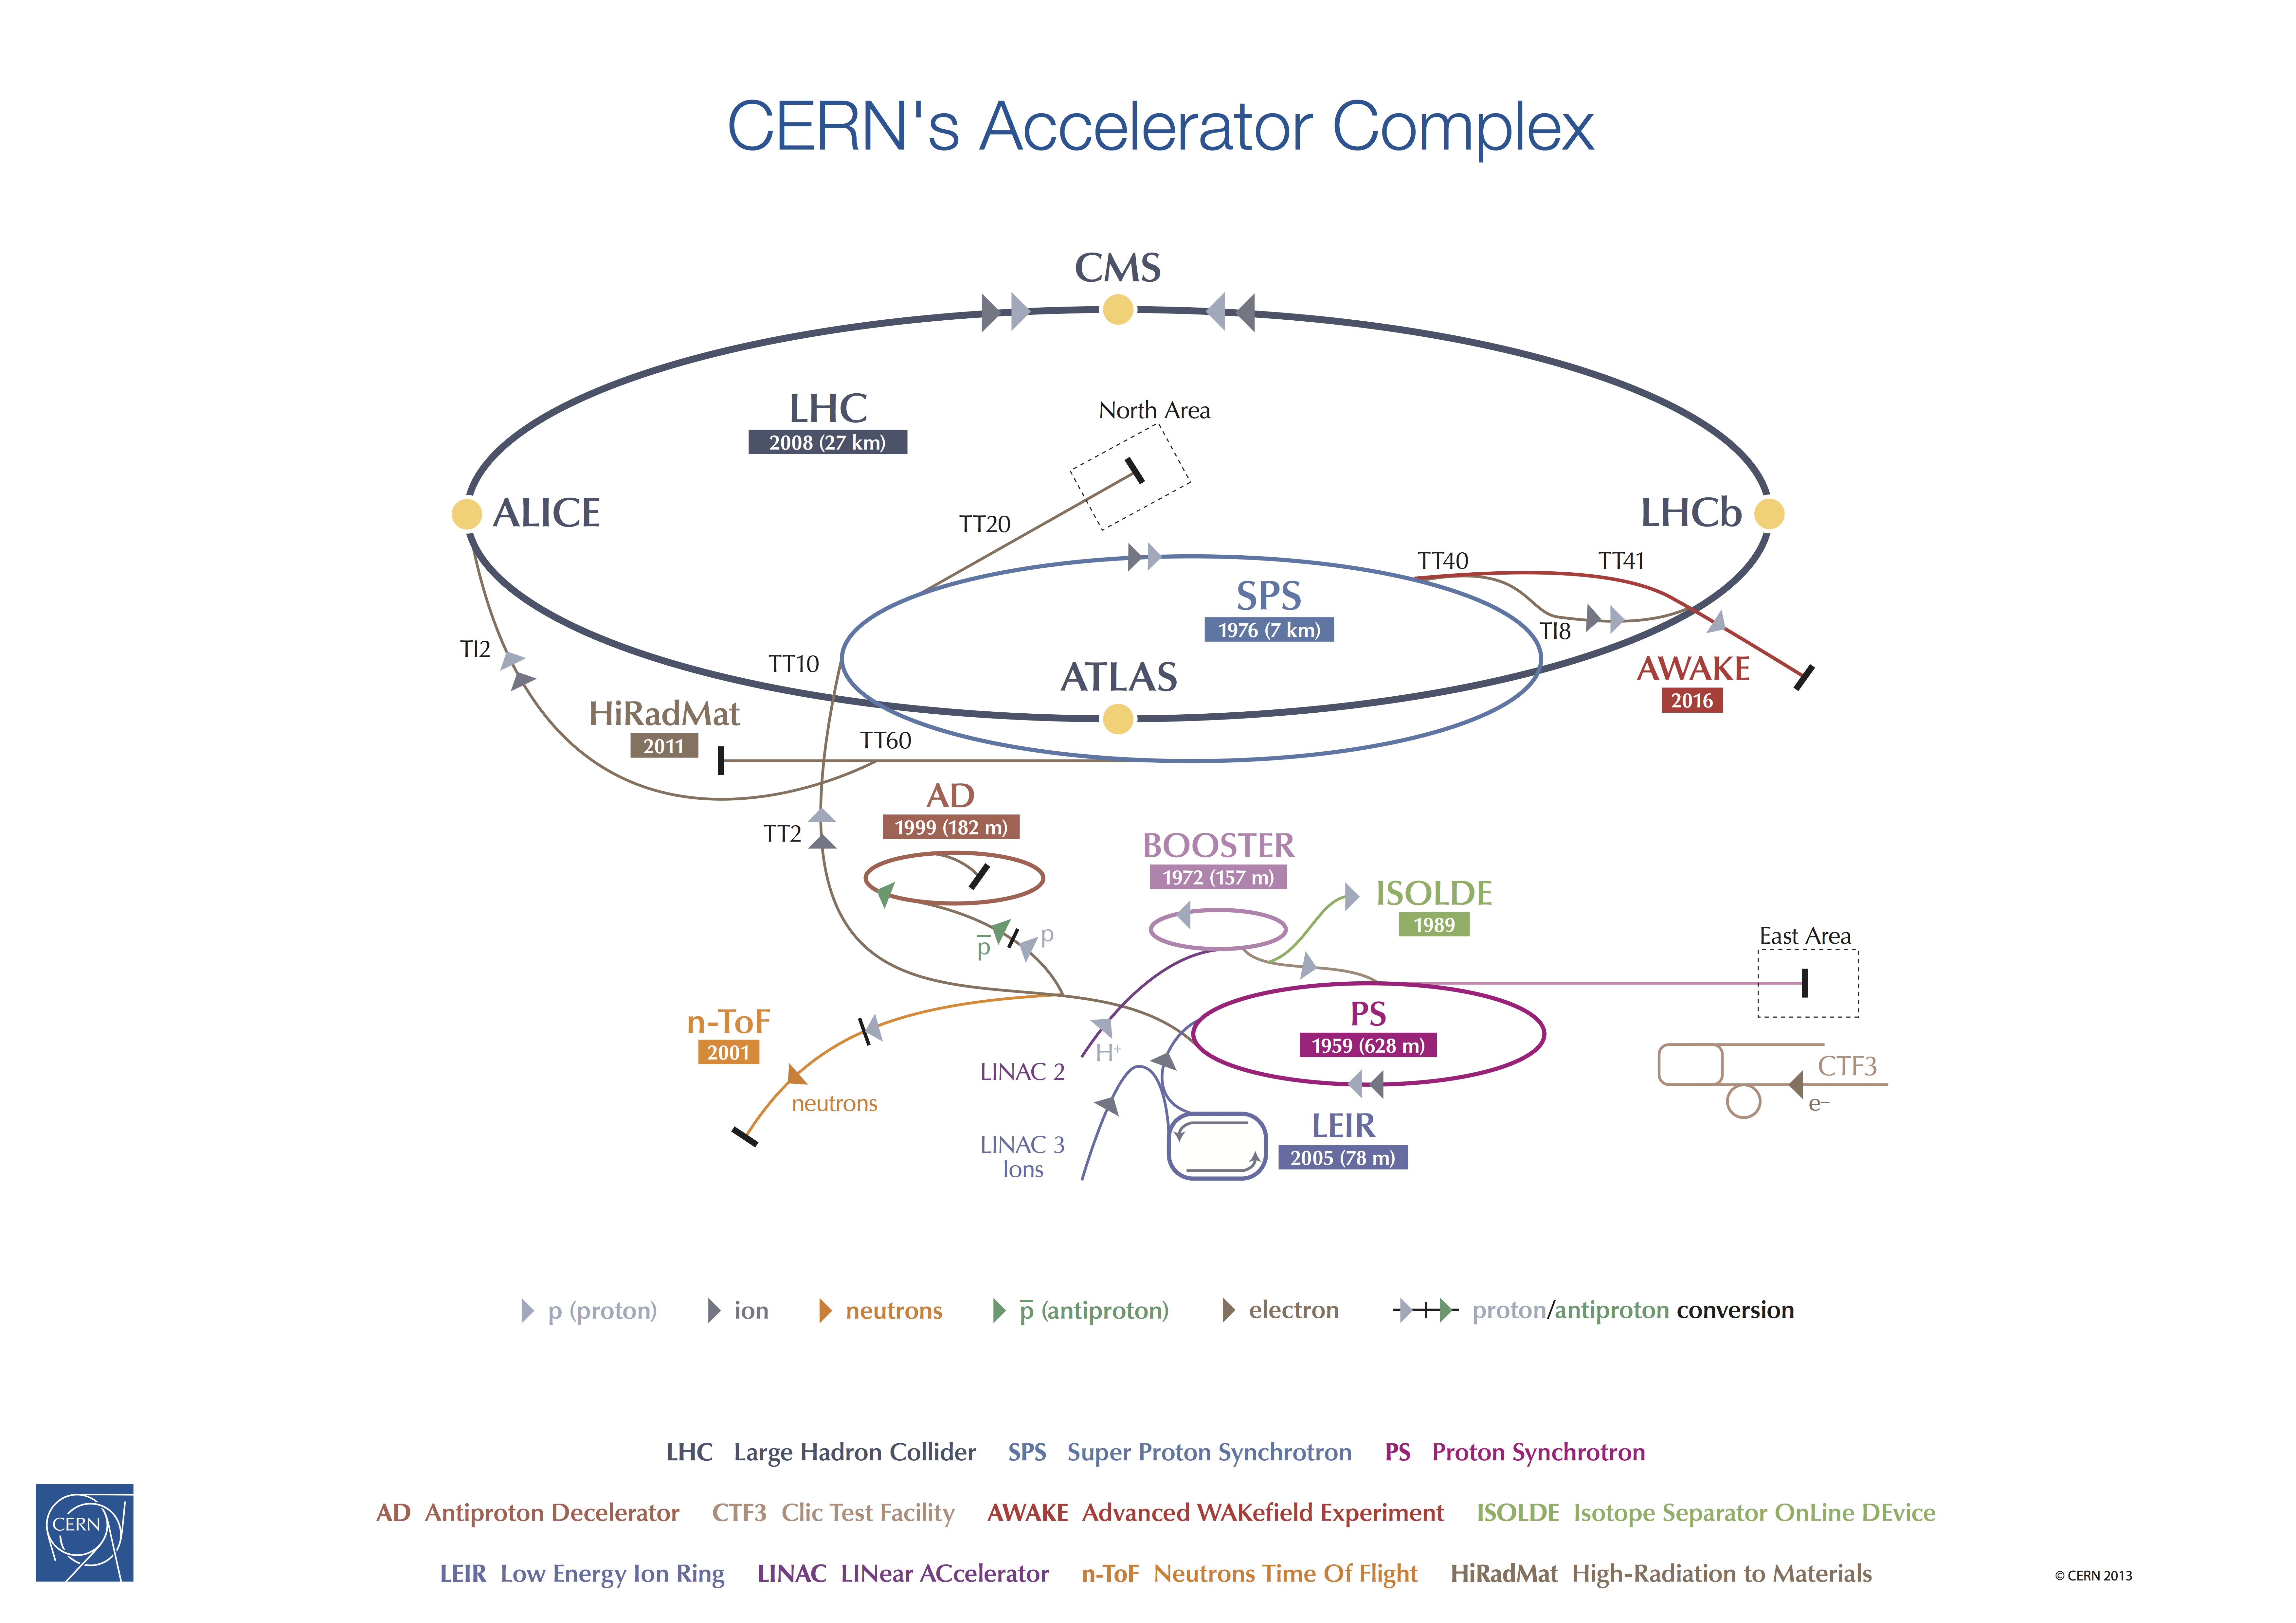
\includegraphics[width=0.9\linewidth]{figures/lhc/injection.jpg}
    \caption{ CERN accelerator complex} 
    \label{fig:injection_chain} 
  \end{center} 
\end{figure}

We begin with the most common element in the Universe, hydrogen, as our source
of protons.  A bottle of hydrogen gas provides 100 microsecond pulses of raw
$H_{2}$ which is then injected into a Duoplasmatron. There,  a strong electric
field and free elctrons from a cathode ionize the molecule into bare $H^{+}$
aka a proton!  These protons are then accelerated by a 90kV electric field,
leaving the Duoplasmatron at 1.4\% the speed of light ($\sim$4000km/s) or, in
Particle Physics units, about 83KeV. The bare protons are then fed into the
accelerating Radio Frequency (RF) cavities of Linear Accelerator 2 (LINAC2).
Inside, conductors charged by a powerful oscillating electromagnetic field
accelerate the protons to an energy of 50MeV. Along the way, small
quadrupole magnets shape the proton bunch ensuring they remain in a tight
beam.  This pattern of acceleration with RF cavities and shaping/tuning with
magnets is then repeated with CERN's first synchrotron, the Proton Synchrotron
(PS) rendering a 1.4 GeV proton beam.  The final step before the LHC comes with the
Super Proton Synchrotron where the same technologies are implemented to produce
450 GeV protons, ready for injection into the LHC. A diagrammatic representation
of this chain can be seen in \Cref{fig:injection_chain}. 

In order to produce proton-proton collisions, the LHC uses two beams
circulating in opposite directions.  The beams are not continuous, but instead
consist of bunches of $\mathcal{O}(10^{11})$ protons with a spacing of 25ns.
Given the LHC circumference this allows for 3564 bunches, however only 2808 are
filled per beam due to safety requirements and injection limitations.  Each
beam takes 4 minutes and 20 seconds to fill and then an additional 20 minutes
to for the protons to reach their maximum energy of 7 TeV, or 99.99999991\%
the speed of light! Under normal operating conditions these beams can be used
for many hours.

\section{LHC Layout and Design} \label{sec:lhc:layout}

While often depicted as a perfect circle the LHC is in reality an octagon with
rounded edges, called arcs, as can be seen in \Cref{fig:lhc_schematic}.
The counter-circulating beams of protons are depicted in red and
blue.  These beams are focused and collided at the 4 dedicated interaction
points at rates of up to 40 MHz.  Two of these points are occupied by the
ATLAS and CMS experiments, both of which are high luminosity, multi-purpose
experiments.

\begin{figure}[!htbp] 
  \begin{center}
    \includegraphics[width=0.9\linewidth]{figures/lhc/lhc_schematic.jpg}
    \caption{Labeled diagram of all the experiments at the LHC indicating the
counter-circulating beams and the relative location of each major experiment
along the circumference of the accelerator \cite{BATTISTONI:2011ujk}.} 
    \label{fig:lhc_schematic} 
  \end{center} 
\end{figure}

The exact design of the LHC tunnel is due to the experimental constraints of the
original machine for which it was built, the Large Electron Positron (LEP)
Collider.  For the $\sim 2,000$ times lighter electron the maximum energy was
limited by synchrotron radiation, proportional to $\frac{1}{m^4}$, requiring
long straight sections of accelerating RF cavities to recuperate the lost
energy.  Because this effect is $\mathcal{O}(10^{13})$ times smaller for the
proton, the LHC is instead limited by the ability to design and construct magnets
strong enough to bend the beam given the already determined curvature of the 8
arcs.

\begin{figure}[!htbp] 
  \begin{center}
    \includegraphics[width=0.9\linewidth]{figures/lhc/dipole.jpg}
    \caption{ Depiction of a LHC dipole magnet 2-in-1 design labeling the major
components \cite{Dailler:842530}.} 
    \label{fig:dipole} 
  \end{center} 
\end{figure}

The oppositely circulating beams must each have their own ring and magnetic field
which led to the creation of a twin-bore (i.e. ``two-in-one") magnet design, a
cross section of which can be seen in \Cref{fig:dipole}. These magnets are constructed
using NbTi superconductors which are cooled to 2 K using superfluid helium.
These magnets are design to provide the needed 8.33 T magnetic field required
to bend the proton trajectories at the designed beam energy of 7 TeV.  In total 1231 of these 15
m bending dipole magnets are used, in association with 392 5-7 m
quadrupole magnets which are responsible for keeping the proton bunches in a
tight beam by squeezing them both horizontally and vertically.

\section{Performance} \label{sec:lhc:performance}

Since the begining of its stable running in 2010 the LHC has performed well,
exceeding expectations.  While the LHC operation itself is incredibly complex,
the performance of the machine, for the purposes of analysis, can be reduced to
three numbers; the familiar center of mass energy of the beams, the integrated
luminosity and the instantaneous luminosity.  

For particle physics the integrated luminosity is proportional to the total
number of collisions recorded during a specified time period, while the
instantaneous luminosity is a function of the number of protons per bunch, the
bunch crossing rate and the cross section of a proton-proton interaction and
represents the particle flux.  Knowing this one can see that the integrated
luminosity, $L_{\text{int}}$ is simply the integral of the instantaneous luminosity
$L_{\text{inst.}}$ for a chosen data period as seen in
\Cref{eq:integrated_luminosity}.

\begin{equation} \label{eq:integrated_luminosity}
   L_{\text{int}} = \int L_{\text{inst.}}dt 
\end{equation}

For a standard Gaussian beam, $L_{\text{inst.}}$ can be written as

\begin{equation} \label{eq:inst_luminosity}
  L_{\text{inst.}} = \frac{N_{b}^{2}n_{b}f_{\text{rev}}\gamma_{r}}{4\pi\epsilon_{n}\beta^{*}}F
\end{equation}

where $N_{b}$ is the number of particles per bunch, $n_{b}$ the number of
bunches per beam, $f_{\text{rev}}$ the revolution frequency, $\gamma_{r}$ the
relativistic gamma factor, $\epsilon_{n}$ the normalized transverse beam
emittance, $\beta^{*}$ the beta function at the collision point, and $F$ the
geometric luminosity reduction factor due to the crossing angle at the
interaction point given by

\begin{equation}
  F = \bigg(1 + \Big( \frac{\theta_{c}\sigma_{z}}{2\sigma^{*}} \Big) ^{2}
\bigg)^{-1/2} 
\end{equation}

where $\theta_{c}$ is the full crossing angle at the interaction point,
$\sigma_{z}$ is the RMS bunch length, and $\sigma^{*}$ is the transverse RMS
beam size at the interaction point \cite{Evans:2008zzb}. Nominal values for the
above quantities are shown in \Cref{table:nominal_values} which also
demonstrates the incredible success of the LHC operators and accelerator teams
during the LHC Run II data taking period.

\begin{table}[htpb]
 \centering
 \caption{
  Nominal design values of LHC operations parameters at ATLAS for $25~\textrm{ns}$ bunch crossing spacing~\cite{Evans:2008zzb,PhysRevAccelBeams.19.101003}.
  Design and ATLAS recorded values of the machine luminosity are also given for LHC Run II operations~\cite{TWiki:2018ATLASPeakLumi}.
 }
 \begin{tabular}{@{}llr@{}} \toprule
  Parameter                                   & Symbol             & LHC Run II Value                \\ \midrule
  LHC circumference                           &                    & $26,659~\mathrm{m}$             \\
  LHC design beam energy                      &                    & $7~\TeV$                        \\
  LHC beam energy in Run II                   &                    & $6.5~\TeV$                      \\
  Number of protons per bunch                 & $N_{b}$            & $1.15 \times 10^{11}$           \\
  Number of proton bunches per beam           & $n_{b}$            & $2,808$                         \\
  Revolution frequency                        & $f_{\textrm{rev}}$ & $11.245~\mathrm{kHz}$           \\
  Lorentz factor (design)                     & $\gamma_{r}$       & $7462.69$                       \\
  Lorentz factor at $\sqrt{s} = 13~\TeV$      &                    & $6929.64$                       \\
  Normalized transverse beam emittance        & $\epsilon_{n}$     & $3.75~\mu\mathrm{m}$            \\
  Collision point beta function               & $\beta^{*}$        & $0.55~\mathrm{m}$               \\
  Full crossing angle                         & $\theta_{c}$       & $285~\mu\mathrm{rad}$           \\
  RMS bunch length                            & $\sigma_{z}$       & $7.55\times 10^{-2}~\mathrm{m}$ \\
  Transverse RMS beam size                    & $\sigma^{*}$       & $16.6~\mu\mathrm{m}$            \\ \midrule
  Peak design machine luminosity at $13~\TeV$ & $L_{\text{inst.}}$ & $9~\inb\mathrm{s}^{-1}$         \\
  Peak ATLAS recorded machine luminosity      &                    & $21~\inb\mathrm{s}^{-1}$        \\
  \bottomrule
 \end{tabular}\label{table:nominal_values}
\end{table}

The ATLAS experiment integrated luminosity for each year can be seen in
\Cref{fig:intlumivsyear} along with an example of the instantaneous luminosity
for $2017$ in \Cref{fig:peakLumiByFill} which is used in the presented analysis.

\begin{figure}[!htbp] 
\centering
\subcaptionbox{Integrated Luminosity 2011 - 2018\label{fig:intlumivsyear}}{\includegraphics[width=0.5\textwidth]{figures/lhc/intlumivsyear.pdf}}\hfill
\subcaptionbox{2017 Peak Instantaneous Luminosity\label{fig:peakLumiByFill}}{\includegraphics[width=0.5\textwidth]{figures/lhc/peakLumiByFill.pdf}}\hfill
\caption{Luminosity is monitored as both a running total known as the
integrated luminosity as depicted in (a) and as an instantaneous quantity as
shown in (b) \cite{LuminosityPublicResultsRun2}.}
\label{fig:luminosity} 
\end{figure}


\section{Pile-up at the LHC} \label{sec:lhc:pileup}

Given the large number of protons per bunch and the cross-section of a
proton-proton interaction, the probability to observe multiple interactions per
bunch crossing is quite high.  These multiple-interaction are known as pile-up,
$\mu$ or the time averaged representation $\langle \mu \rangle$, and come in two
different forms: 

\begin{enumerate} \item \textbf{In-time pile-up:} These are the other
proton-proton collisions that occur during the same bunch crossing as the
primary interaction that cauesd the Data Aquisition (DAQ) system to trigger.
These are the standard extra interactions we expect to observe as stated above.
\item \textbf{Out-of-time pile-up:} These are interactions that occur either
before or after a bunch crossing that causes the DAQ to trigger.  This effect is
generally due to the long integration times of some detector electronics.
\end{enumerate}

The pile-up profile for past years can be seen in figure XXX.  The width of this
distributino is due a combination of Poisonian statistics, the decrease in
number of protons per bunch over the lifetime of a single run, and optimization
tweaks to the beam's profile during runtime.  Understanding and eliminating the
noise from these pile-up events is crucial to reconstructing physics variables
to represent the primary interaction we hope to observe.

